\documentclass[11pt]{article}

\usepackage[utf8]{inputenc}
\usepackage[margin=1in]{geometry} 
\usepackage{amsmath,amsthm,amssymb,graphicx,mathtools,tikz,hyperref,multicol,cancel,enumitem,booktabs,float,pgfplots,multirow,mathrsfs,textcomp,gensymb,soul,changepage,threeparttable}
%\usepackage[table]{xcolor}
\usepackage[T1]{fontenc}
\usepackage[italian]{babel}
\usepackage{hyphenat}
\usepackage{subfig}
\hyphenation{mate-mati-ca recu-perare}
\usetikzlibrary{positioning}
\pgfplotsset{compat=1.14}

\newcommand{\n}{\mathbb{N}}
\newcommand{\z}{\mathbb{Z}}
\newcommand{\q}{\mathbb{Q}}
\newcommand{\cx}{\mathbb{C}}
\newcommand{\real}{\mathbb{R}}
\newcommand{\field}{\mathbb{F}}
\newcommand{\ita}[1]{\textit{#1}}
\newcommand{\com}[2]{#1\backslash#2}
\newcommand{\oneton}{\{1,2,3,...,n\}}
\newcommand{\idea}[1]{\begin{gather*}#1\end{gather*}}
\newcommand{\ef}{\ita{f} }
\newcommand{\eff}{\ita{f}}
\newcommand{\proofs}[1]{\begin{proof}#1\end{proof}}
\newcommand{\inv}[1]{#1^{-1}}
\newcommand{\setb}[1]{\{#1\}}
\newcommand{\en}{\ita{n }}
\newcommand{\vbrack}[1]{\langle #1\rangle}
\newcommand{\qRa}{\quad \Rightarrow \quad}
\newcommand{\smaca}[1]{\textbf{\textsc{#1}}}

\newenvironment{theorem}[2][Teorema]{\begin{trivlist}
\item[\hskip \labelsep {\bfseries #1}\hskip \labelsep {\bfseries #2.}]}{\end{trivlist}}
\newenvironment{lemma}[2][Lemma]{\begin{trivlist}
\item[\hskip \labelsep {\bfseries #1}\hskip \labelsep {\bfseries #2.}]}{\end{trivlist}}
\newenvironment{exercise}[2][Esercizio]{\begin{trivlist}
\item[\hskip \labelsep {\bfseries #1}\hskip \labelsep {\bfseries #2.}]}{\end{trivlist}}
\newenvironment{proposition}[2][Proposizione]{\begin{trivlist}
\item[\hskip \labelsep {\bfseries #1}\hskip \labelsep {\bfseries #2.}]}{\end{trivlist}}
\newenvironment{corollary}[2][Corollario]{\begin{trivlist}
\item[\hskip \labelsep {\bfseries #1}\hskip \labelsep {\bfseries #2.}]}{\end{trivlist}}

\hypersetup {
    colorlinks,
    linkcolor=blue
}

\graphicspath{{img/}}

\begin{document}
\setlength{\parindent}{0pt}
\title{\vspace{-4em}{\large Laboratorio di Meccanica e Termodinamica} \\
    Relazione di Laboratorio}
\author{GRUPPO 3 \\
    Gerardo Selce, Maurizio Liguori, Emanuela Galluccio, Francesco Messano}
\date{12/11/2024}
\maketitle

\vspace{-2em}\par\noindent\rule{\textwidth}{0.4pt}
\begin{center}
    {\Large\sc Piano inclinato - Guida a cuscino d'aria}  
\end{center}
\par\noindent\rule{\textwidth}{0.4pt}
\section{Introduzione}

Obiettivo dell’esperimento è determinare indirettamente l’accelerazione di un corpo che si muove lungo un piano inclinato. Il piano è stato posizionato con cinque diverse inclinazioni e, per ciascuna di esse, è stata calcolata la velocità media del corpo su sei diverse lunghezze, applicando la formula

Scopo dell'esperienza è la misurazione indiretta dell'accelerazione di un corpo che si muove lungo un piano inclinato. Il piano è stato posto a cinque diverse inclinazioni dopodichè, per ognuna di esse, è stata misurata la velocità media del corpo per sei lunghezze utilizzando la legge:
\begin{equation}
    \overline{v}=\frac{\Delta s}{t}
\end{equation}
Per ogni ampiezza del piano inclinato è stato costruito un grafico della velocità media in funzione del tempo e tracciando la retta di regressione, è stato possibile ricavare il valore dell'accelerazione. Infine è stato tracciato un ultimo grafico che mette in relazione l'accelerazione del corpo in funzione del seno dell'angolo di inclinazione del piano.

\section{Richiami teorici}

Il piano inclinato è essenzialmente una superficie piatta inclinata di un angolo $\alpha$ rispetto al piano orizzontale. Quando un corpo di muove lungo il piano, le forze che agiscono sono:
\begin{enumerate}
    \item \textbf{La forza gravitazionale} ($mg$), che agisce lungo la verticale.
    \item \textbf{La componente perpendicolare alla superficie} ($mg\cos(\alpha)$) che mantiene l'oggetto premuto contro il piano e non contribuisce al moto.
    \item \textbf{La componente parallela al piano} ($mg\sin(\alpha)$) che causa il moto lungo il piano.
\end{enumerate}
L'oggetto inizierà a muoversi solo quando la componente parallela ($mg\sin(\alpha)$) supera in intensità l'attrito statico. Una volta in moto, l'accelerazione impressa dalla gravità viene smorzata per effetto dell'attrito dinamico. Poichè l'accelerazione di un corpo su un piano inclinato è costante in assenza di forze esterne, il suo moto può essere descritto attraverso la legge oraria del moto uniformemente accelerato:
\begin{equation}
    s(t)=s_o+v_0t+\frac{1}{2}at^2
\end{equation}
Spostando il termine $s_0$ al primo membro e dividendo entrambi i membri per $t$ si ottiene la velocità media descritta dalla Legge (1), la quale corrisponde a:
\begin{equation}
    \overline{v}=v_0+\frac{1}{2}at
\end{equation}
La velocità media in funzione del tempo sarà quindi descritta da una retta la cui intercetta sarà $v_0$ (velocità iniziale del corpo) e il cui coefficiente angolare sarà $\frac{a}{2}$.

\section{Descrizione dell'apparato sperimentale}

Per svolgere questa esperienza è stato utilizzato il seguente apparato sperimentale:
\begin{itemize}
    \item Rotaia a cuscino d'aria
    \item Carrello per la rotaia
    \item Due celle fotoelettriche
    \item Elettrocalamita
    \item Metro a nastro 
    \item Cronometro digitale
    \item Compressore d'aria
\end{itemize}

\begin{table}[H]
\centering
\begin{tabular}{|c|c|}
\hline
\textbf{Strumenti di misura} & \textbf{Risoluzione} \\
\hline
Metro a nastro & $1\ mm$ \\
Cronometro digitale & $0.01\ s$ \\
\hline
\end{tabular}
\caption{Risoluzione degli strumenti di misura utilizzati}
\label{tab:}
\end{table}

\begin{figure}[H]
  \centering
  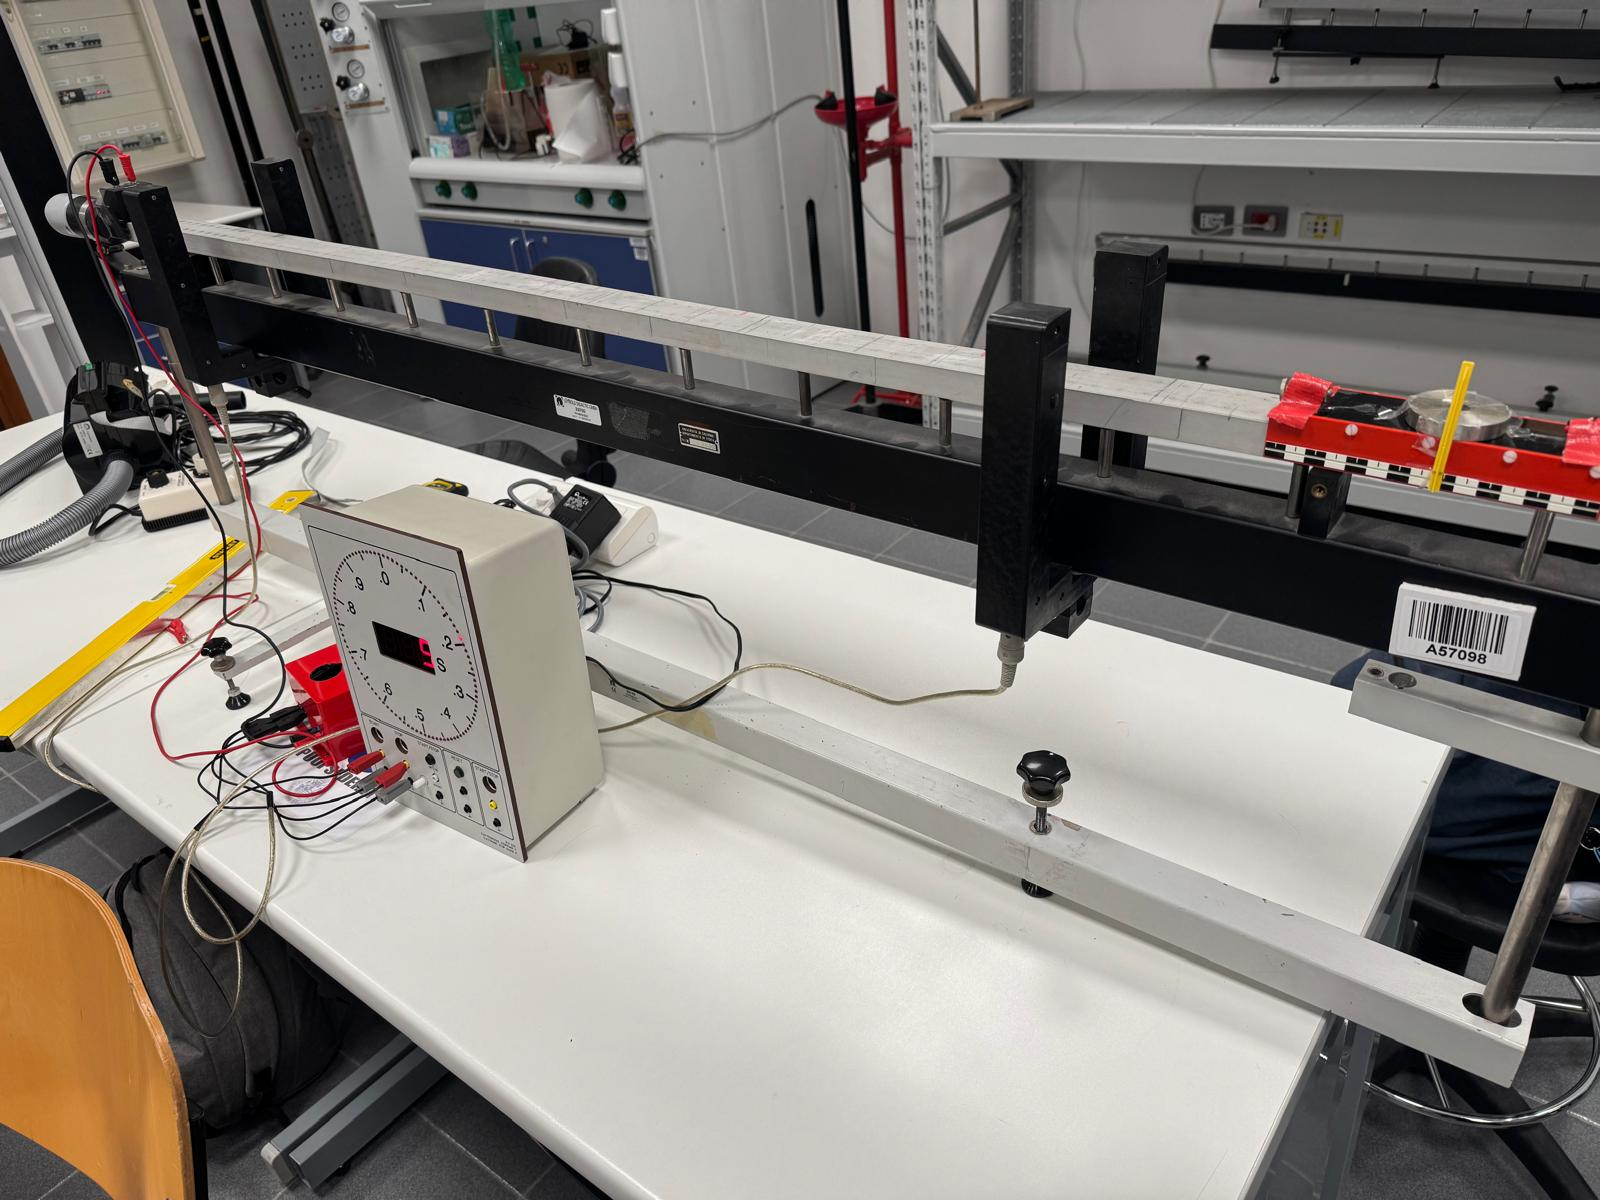
\includegraphics[width=0.75\textwidth]{piano inclinato.jpg}
  \caption{Piano inclinato composto dalla rotaia a cuscino d'aria, carrello, due celle fotoelettriche ed elettrocalamita.}
\end{figure}



\begin{figure}[H]
  \centering
  \subfloat[Cronometro digitale]{%
    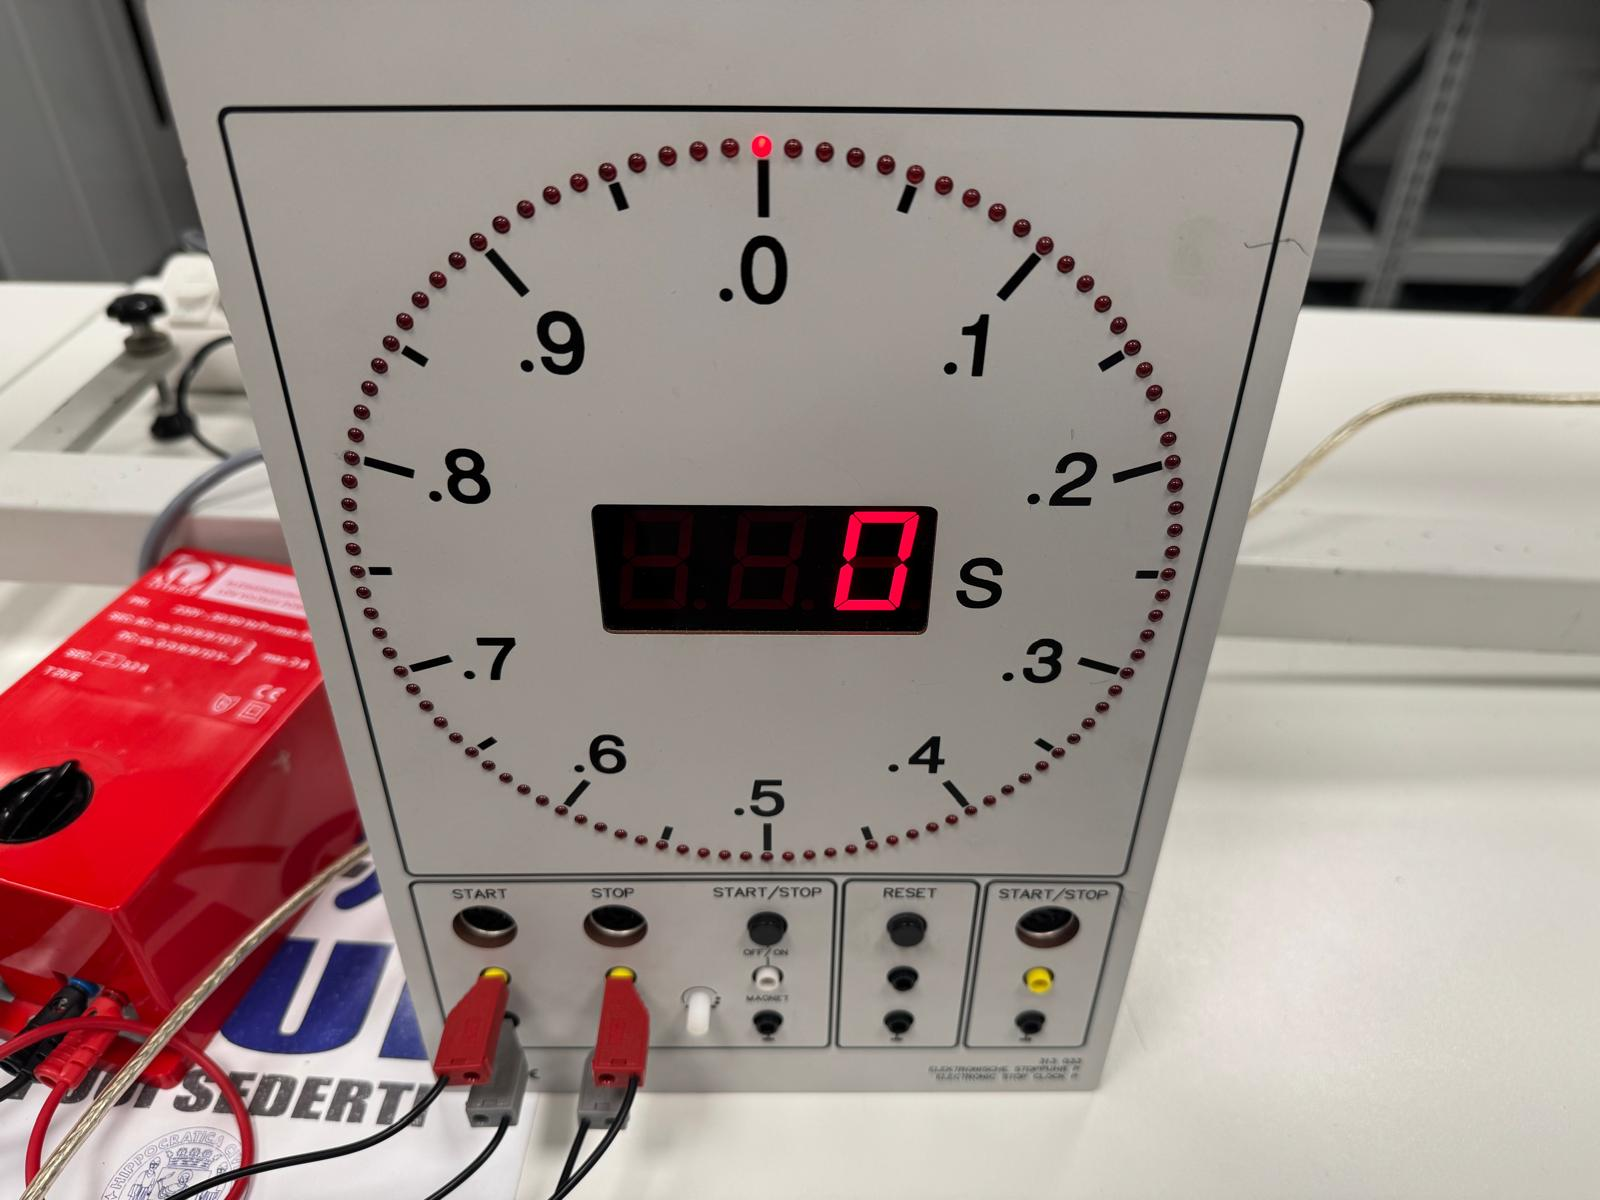
\includegraphics[width=0.45\textwidth]{cronometro.jpg}
  }
  \hspace{0.5cm} % Spazio tra le due immagini
  \subfloat[Metro a nastro]{%
    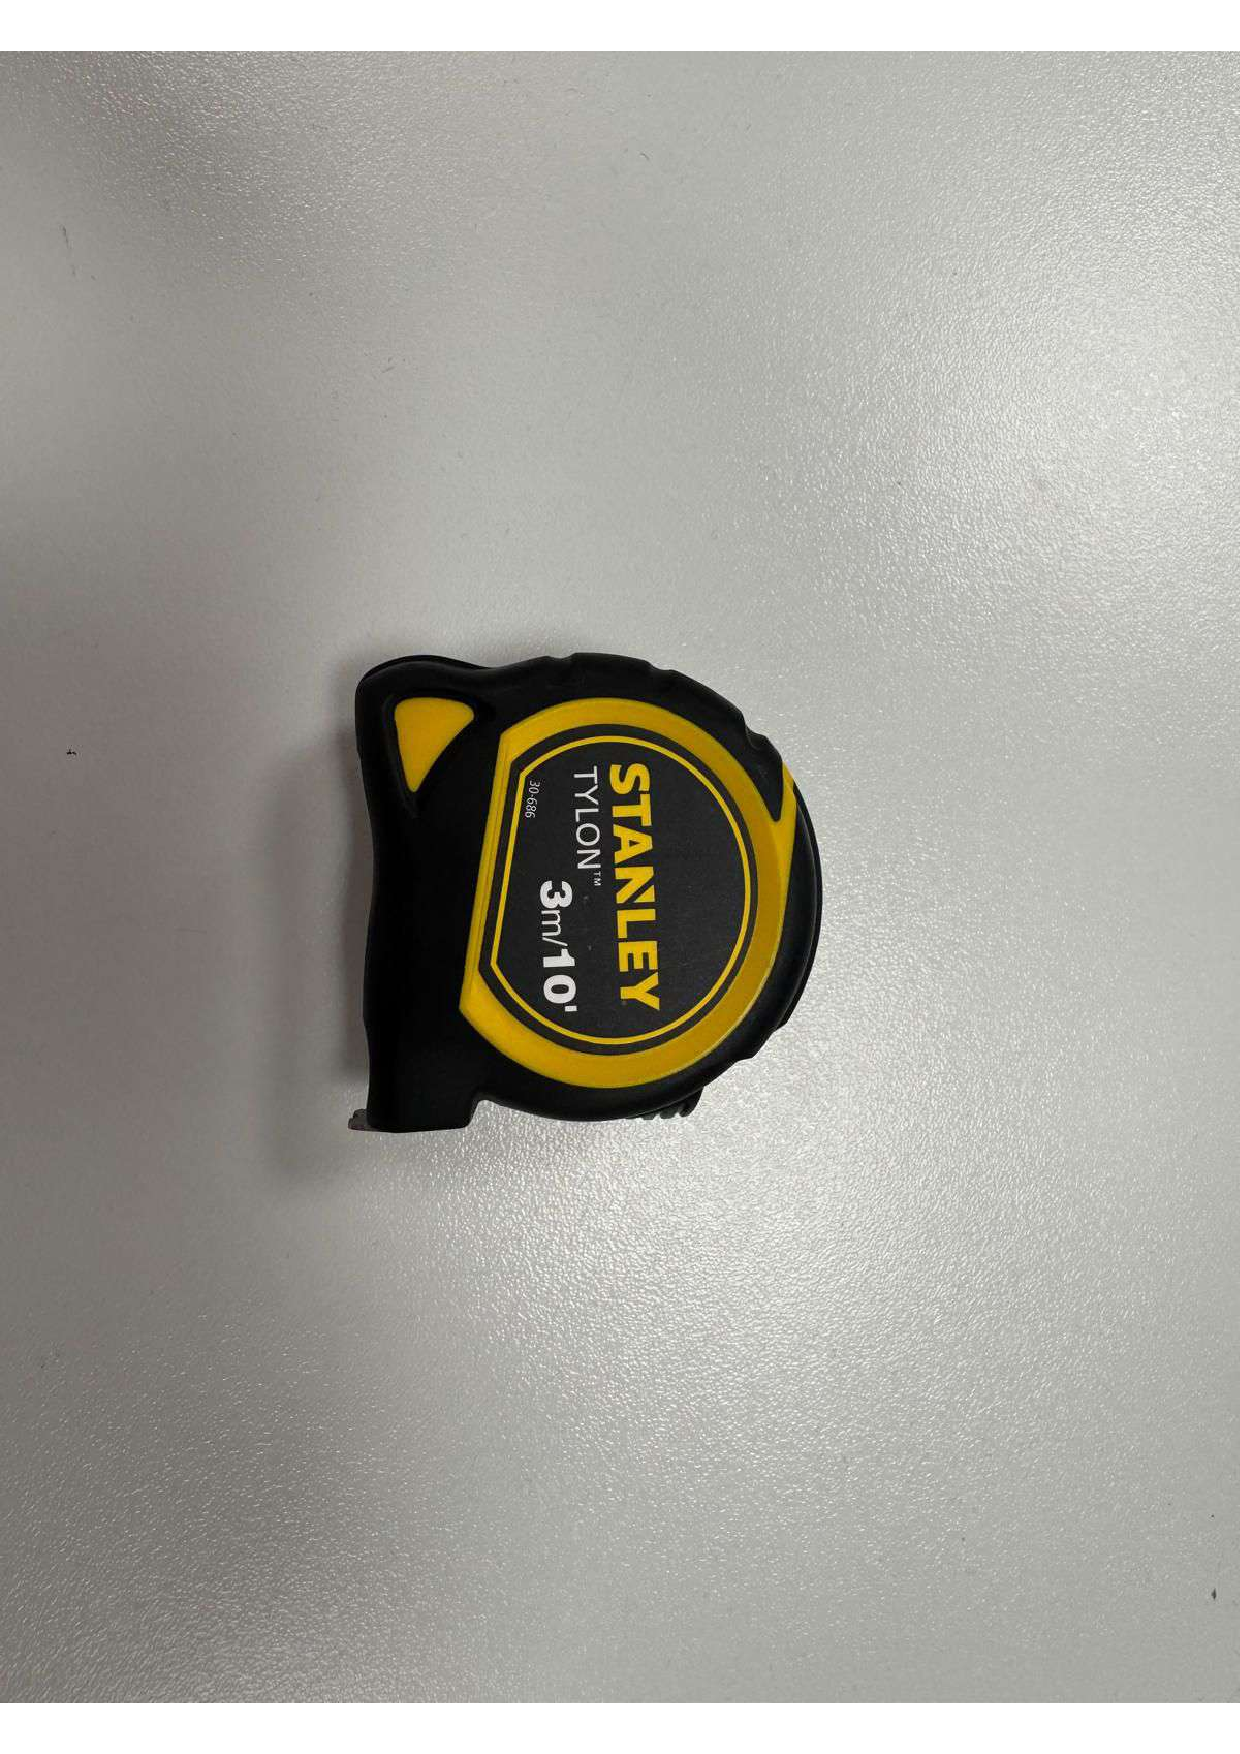
\includegraphics[width=0.45\textwidth]{metro.pdf}
  }
  \label{fig:due_immagini}
\end{figure}

\begin{figure}[H]
  \centering
  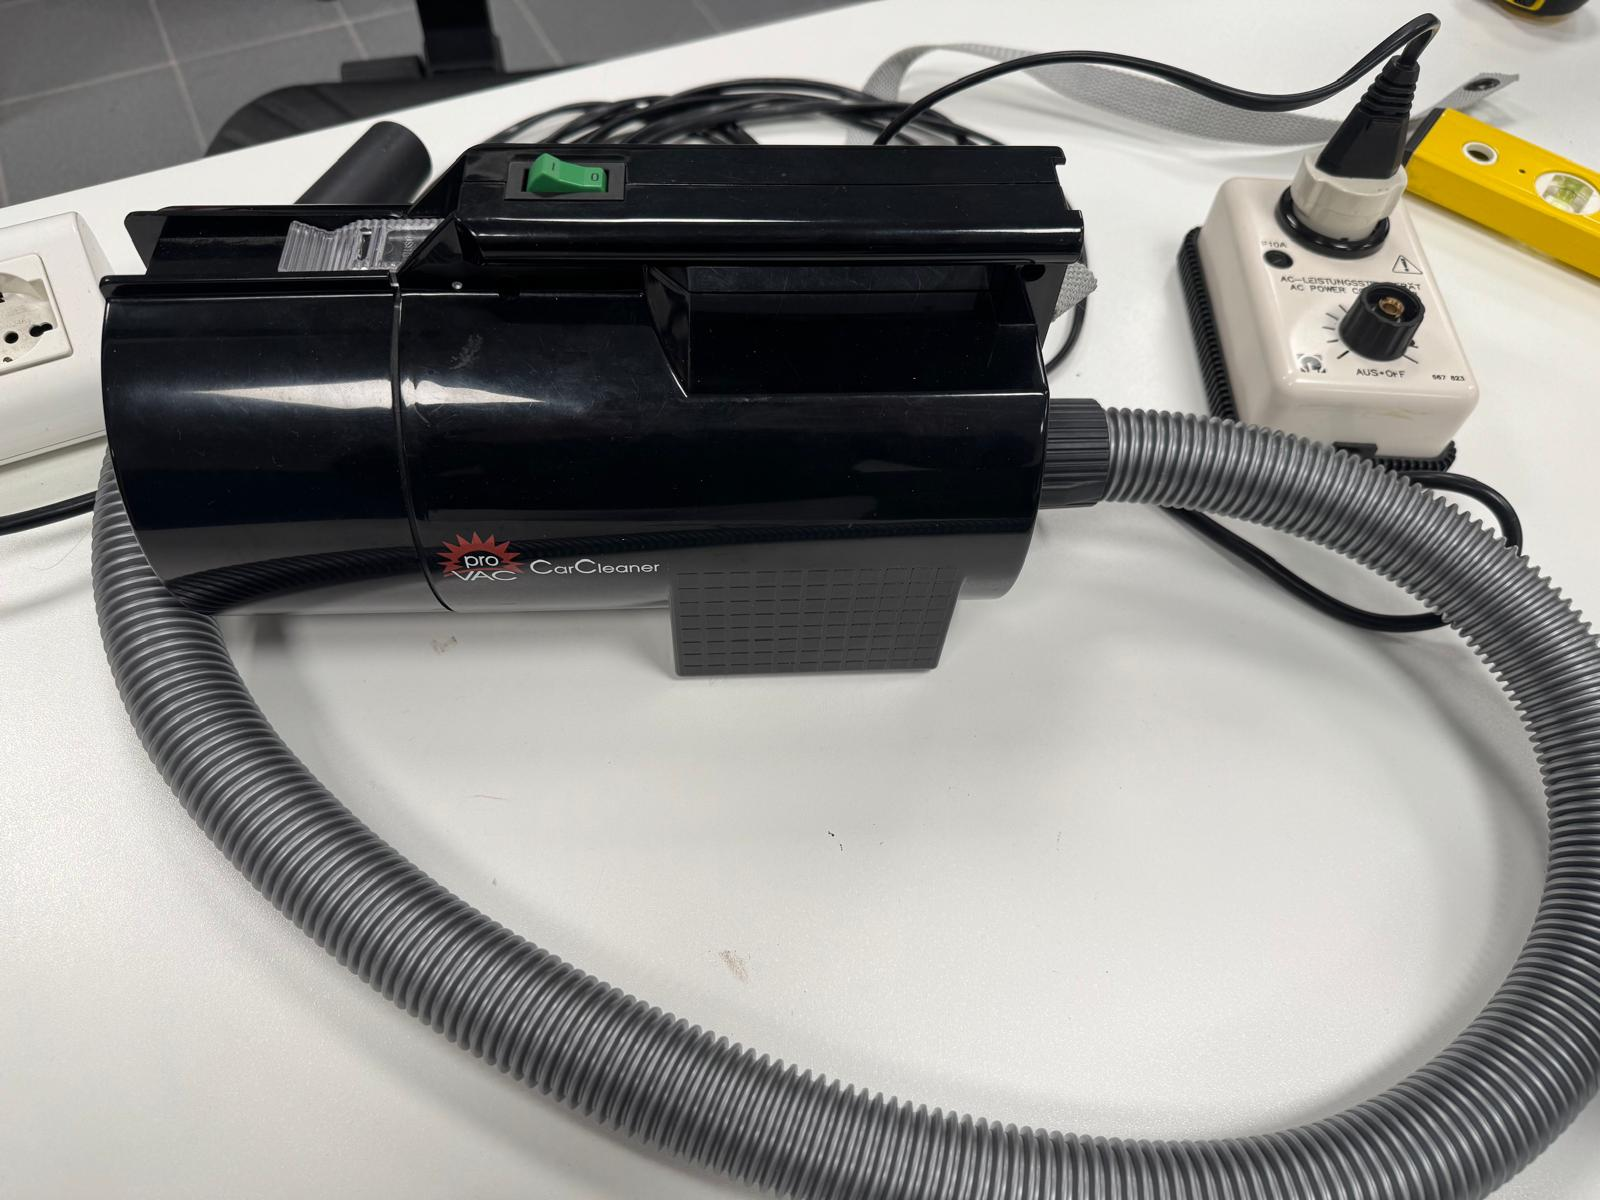
\includegraphics[width=0.55\textwidth]{aria.jpg}
  \caption{Compressore d'aria utilizzato per generare il cuscino d'aria intorno al piano inclinato e permettere al corpo di scivolare minimizzando il coefficiente di attrito statico.}
\end{figure}

\section{Descrizione e analisi dei dati sperimentali}

Considerato un triangolo rettangolo in cui l'ipotenusa rappresenta il piano inclinato, abbiamo misurato dell'angolo $\alpha$ utilizzando la formula
\begin{equation}
    \alpha=\arctan(\frac{C_1}{C_2})
\end{equation}
In cui $C_1$ è l'altezza e $C_2$ la base.
L'inclinazione del piano può essere modificata attraverso la rotazione di una manovella. Una rotazione completa corrisponde alla variazione di $1\ mm$ di $C1$ lungo la verticale. Sono state misurate cinque diverse inclinazioni, che corrispondo a cinque diversi valori di $C_1$. L'incertezza è trascurata.
\begin{table}[H]
\centering
\begin{tabular}{|c|c|}
\hline
\textbf{N°} & \textbf{$C_1$ ($cm$)} \\
\hline
$1$ & $0.5$ \\
$2$ & $1.0$ \\
$3$ & $1.5$ \\
$4$ & $1.9$ \\
$5$ & $2.3$ \\
\hline
\end{tabular}
\caption{Valori di $C_1$}
\label{tab:}
\end{table}
Utilizzando il metro a nastro abbiamo misurato $C_2=(85\pm 0.05)\ cm$. Si noti che la lunghezza di $C_2$ è costante. \\
Per ogni ampiezza sono state prese in considerazione sempre le stesse sei $\Delta s$, misurate utilizzando il metro a nastro. \\
\begin{table}[H]
\centering
\begin{tabular}{|c|c|}
\hline
\textbf{N°} & \textbf{$\Delta s$ ($m$)} \\
\hline
$1$ & $0.2165\pm 0.0005$ \\
$2$ & $0.3500\pm 0.0005$ \\
$3$ & $0.4800\pm 0.0005$ \\
$4$ & $0.6100\pm 0.0005$ \\
$5$ & $0.7800\pm 0.0005$ \\
$6$ & $0.9400\pm 0.0005$ \\
\hline
\end{tabular}
\caption{Valori di $\Delta s$}
\label{tab:}
\end{table}
Fissata un'ampiezza $\alpha_i$, per ogni lunghezza $\Delta s_i$ la misurazione del tempo è stata effettuata tre volte. Il valore finale è stato stimato come punto medio tra la misura più piccola e più grande ottenute, mentre l'incertezza sulla misura è stata valutata con la semidispersione, poichè il suo valore risulta maggiore della risoluzione strumentale. Nel calcolo di $\overline{v_i}$ è stata tenuta in considerazione la propagazione dell'errore strumentale che affligge le misurazioni di lunghezza e tempo.

\subsection{Ampiezza $\alpha_1=0.00588\ rad$}
\begin{table}[H]
\centering
\begin{tabular}{|c|c|}
\hline
\textbf{$t$ ($s$)} & \textbf{$\overline{v}$ ($\frac{m}{s}$)} \\
\hline
$1.28\pm 0.01$ & $0.1691\pm 0.0017$ \\
$1.80\pm 0.01$ & $0.1944\pm 0.0014$ \\
$2.23\pm 0.01$ & $0.2153\pm 0.0012$ \\
$2.61\pm 0.01$ & $0.2337\pm 0.0011$ \\
$3.05\pm 0.01$ & $0.2557\pm 0.0010$ \\
$3.45\pm 0.01$ & $0.2725\pm 0.0010$ \\
\hline
\end{tabular}
\caption{$t$ indica il tempo di percorrenza dei rispettivi $\Delta s$ riportati in Tabella (4) e $\overline{v}$ la velocità media.}
\label{tab:}
\end{table}
\begin{figure}[H]
  \centering
  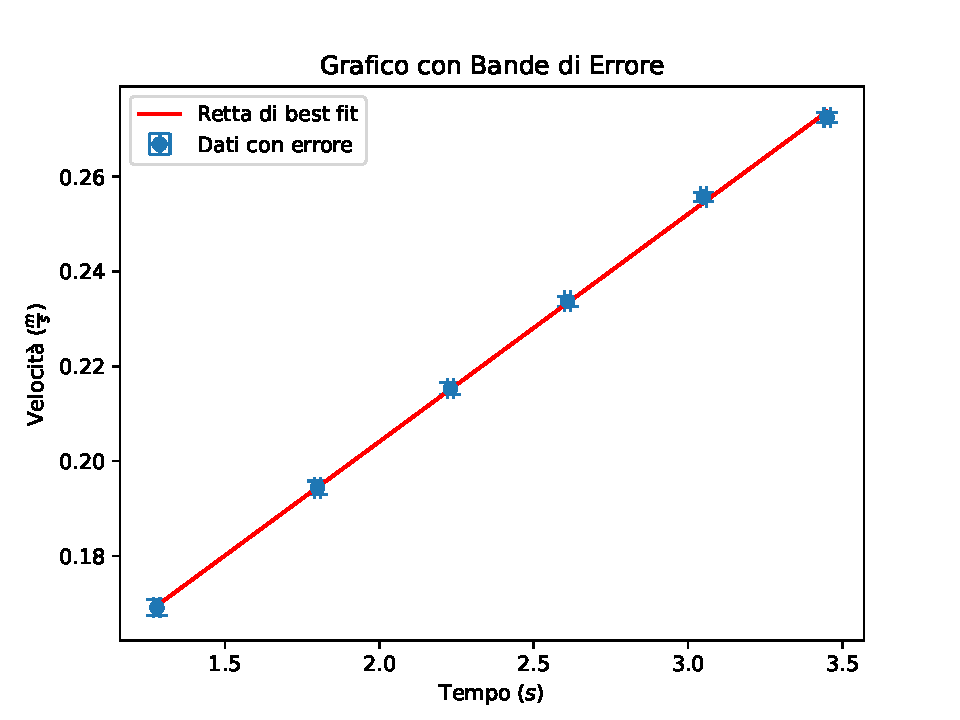
\includegraphics[width=1\textwidth]{grafico1p1.pdf}
  \caption{Grafico della velocità media in funzione del tempo dei valori in Tabella (4). \\
    Coefficiente angolare = ($0.04804\pm 0.00150$) $\frac{m}{s^2}$ (Vedi Legge (5) e (7)).}
\end{figure}

\subsection{Ampiezza $\alpha_2=0.01176\ rad$}
\begin{table}[H]
\centering
\begin{tabular}{|c|c|}
\hline
\textbf{$t$ ($s$)} & \textbf{$\overline{v}$ ($\frac{m}{s}$)} \\
\hline
$0.99\pm 0.01$ & $0.2187\pm 0.0028$ \\
$1.41\pm 0.01$ & $0.2482\pm 0.0022$ \\
$1.73\pm 0.01$ & $0.2775\pm 0.0019$ \\
$2.02\pm 0.01$ & $0.3020\pm 0.0018$ \\
$2.36\pm 0.01$ & $0.3305\pm 0.0017$ \\
$2.65\pm 0.01$ & $0.3547\pm 0.0016$ \\
\hline
\end{tabular}
\caption{$t$ indica il tempo di percorrenza dei rispettivi $\Delta s$ riportati in Tabella (4) e $\overline{v}$ la velocità media.}
\label{tab:}
\end{table}
\begin{figure}[H]
  \centering
  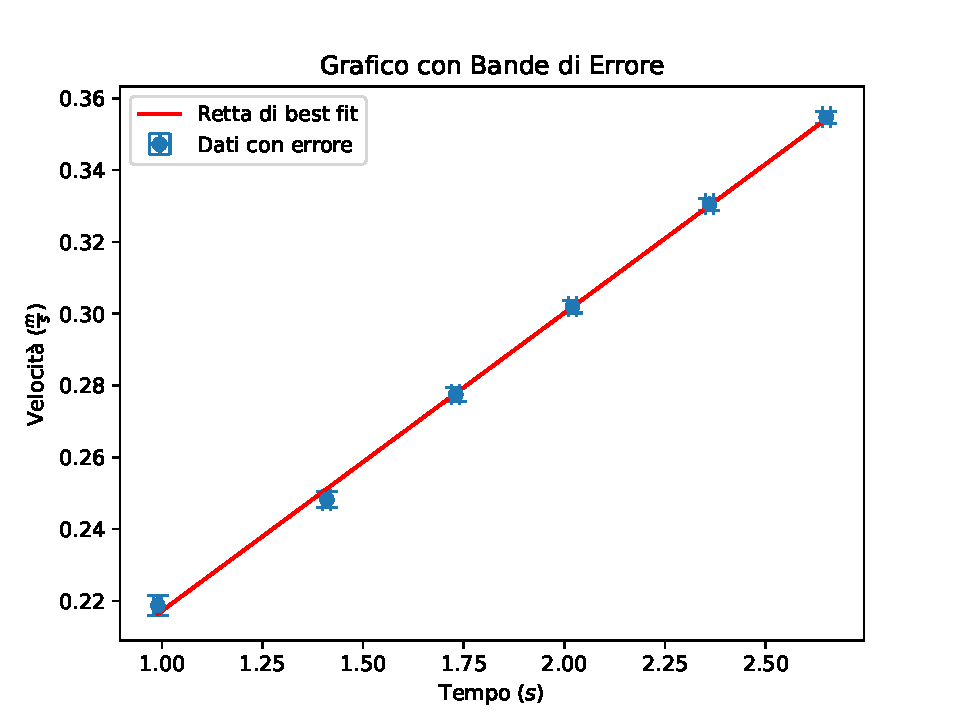
\includegraphics[width=1\textwidth]{grafico2p1.pdf}
  \caption{Grafico della velocità media in funzione del tempo dei valori in Tabella (5). \\
    Coefficiente angolare = ($0.08302\pm 0.00427$) $\frac{m}{s^2}$ (Vedi Legge (5) e (7)).}
\end{figure}

\subsection{Ampiezza $\alpha_3=0.01765\ rad$}
\begin{table}[H]
\centering
\begin{tabular}{|c|c|}
\hline
\textbf{$t$ ($s$)} & \textbf{$\overline{v}$ ($\frac{m}{s}$)} \\
\hline
$0.84\pm 0.01$ & $0.2577\pm 0.0037$ \\
$1.18\pm 0.01$ & $0.2966\pm 0.0030$ \\
$1.46\pm 0.01$ & $0.3288\pm 0.0026$ \\
$1.71\pm 0.01$ & $0.3567\pm 0.0024$ \\
$1.99\pm 0.01$ & $0.3920\pm 0.0023$ \\
$2.24\pm 0.01$ & $0.4196\pm 0.0021$ \\
\hline
\end{tabular}
\caption{$t$ indica il tempo di percorrenza dei rispettivi $\Delta s$ riportati in Tabella (4) e $\overline{v}$ la velocità media.}
\label{tab:}
\end{table}
\begin{figure}[H]
  \centering
  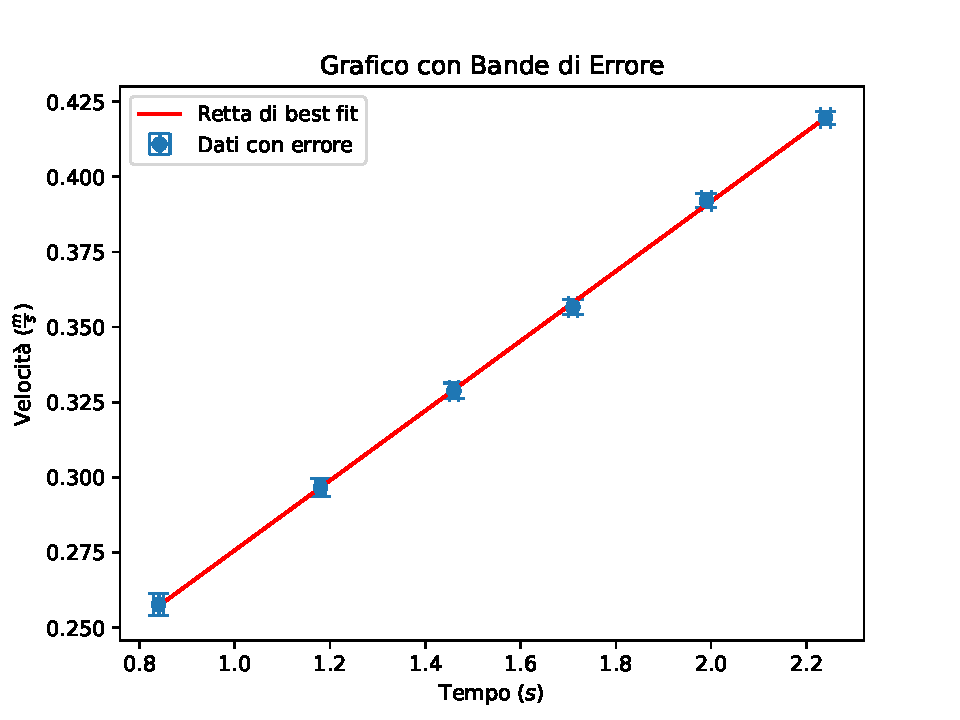
\includegraphics[width=1\textwidth]{grafico3p1.pdf}
  \caption{Grafico della velocità media in funzione del tempo dei valori in Tabella (6). \\
    Coefficiente angolare = ($0.11606\pm 0.00269$) $\frac{m}{s^2}$ (Vedi Legge (5) e (7)).}
\end{figure}

\subsection{Ampiezza $\alpha_4=0.02235\ rad$}
\begin{table}[H]
\centering
\begin{tabular}{|c|c|}
\hline
\textbf{$t$ ($s$)} & \textbf{$\overline{v}$ ($\frac{m}{s}$)} \\
\hline
$0.76\pm 0.01$ & $0.2849\pm 0.0044$ \\
$1.07\pm 0.01$ & $0.3271\pm 0.0036$ \\
$1.30\pm 0.01$ & $0.3692\pm 0.0033$ \\
$1.53\pm 0.01$ & $0.3987\pm 0.0030$ \\
$1.78\pm 0.01$ & $0.4382\pm 0.0028$ \\
$2.00\pm 0.01$ & $0.4700\pm 0.0026$ \\
\hline
\end{tabular}
\caption{$t$ indica il tempo di percorrenza dei rispettivi $\Delta s$ riportati in Tabella (4) e $\overline{v}$ la velocità media.}
\label{tab:}
\end{table}
\begin{figure}[H]
  \centering
  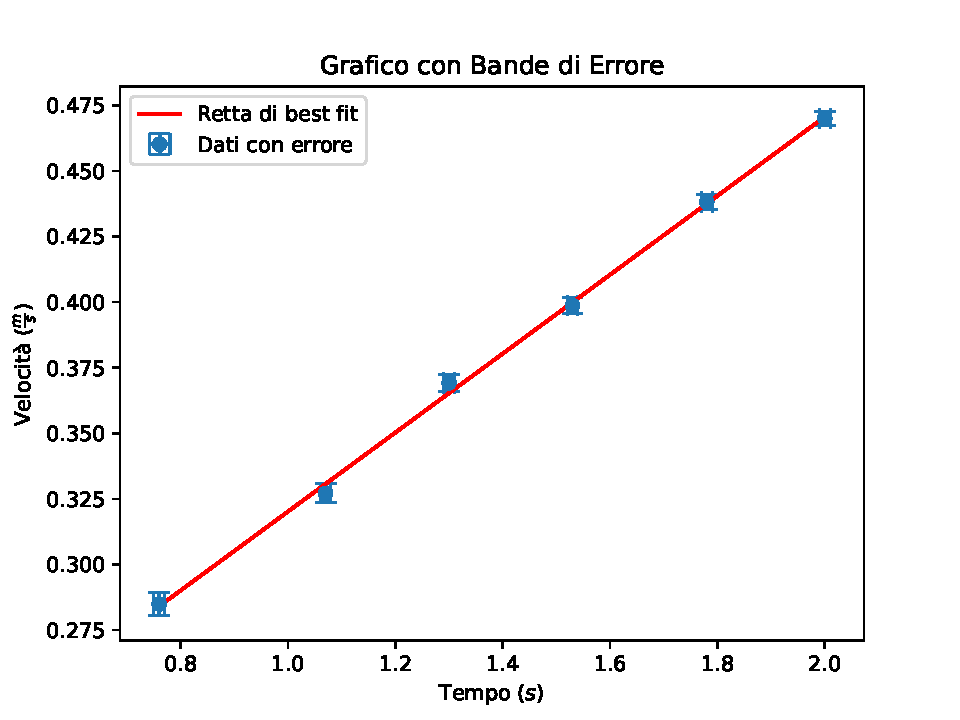
\includegraphics[width=1\textwidth]{grafico4p1.pdf}
  \caption{Grafico della velocità media in funzione del tempo dei valori in Tabella (7). \\
    Coefficiente angolare = ($0.15044\pm 0.00817$) $\frac{m}{s^2}$ (Vedi Legge (5) e (7)).}
\end{figure}

\subsection{Ampiezza $\alpha_5=0.02705\ rad$}
\begin{table}[H]
\centering
\begin{tabular}{|c|c|}
\hline
\textbf{$t$ ($s$)} & \textbf{$\overline{v}$ ($\frac{m}{s}$)} \\
\hline
$0.69\pm 0.01$ & $0.3138\pm 0.0053$ \\
$0.98\pm 0.01$ & $0.3571\pm 0.0042$ \\
$1.20\pm 0.01$ & $0.4000\pm 0.0038$ \\
$1.40\pm 0.01$ & $0.4357\pm 0.0035$ \\
$1.63\pm 0.01$ & $0.4785\pm 0.0033$ \\
$1.83\pm 0.01$ & $0.5137\pm 0.0031$ \\
\hline
\end{tabular}
\caption{$t$ indica il tempo di percorrenza dei rispettivi $\Delta s$ riportati in Tabella (4) e $\overline{v}$ la velocità media.}
\label{tab:}
\end{table}
\begin{figure}[H]
  \centering
  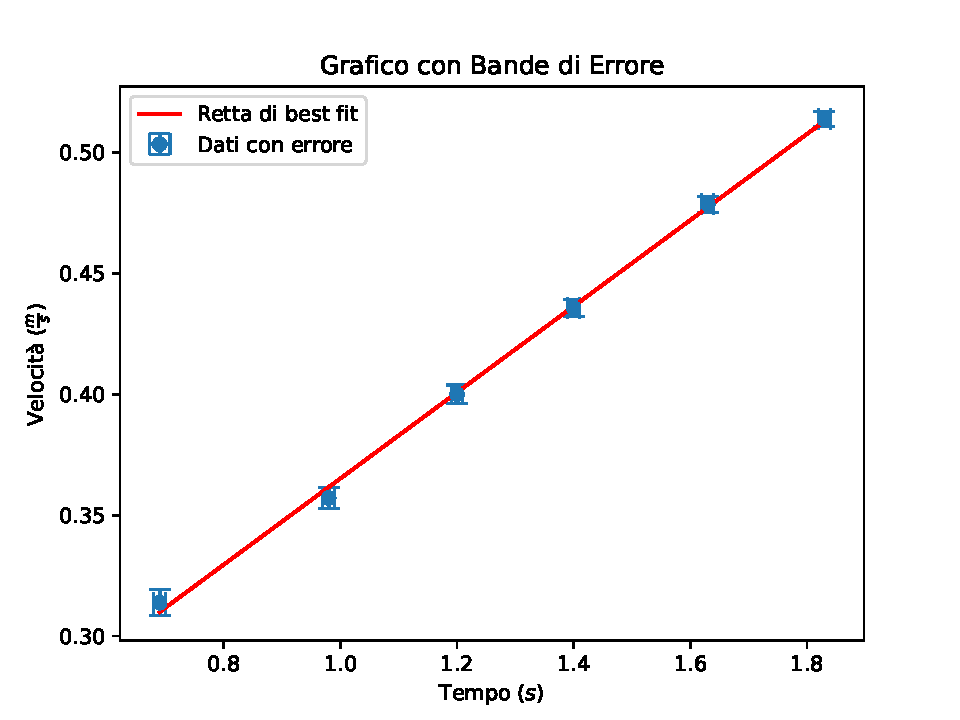
\includegraphics[width=1\textwidth]{grafico5p1.pdf}
  \caption{Grafico della velocità media in funzione del tempo dei valori in Tabella (8). \\
    Coefficiente angolare = ($0.17793\pm 0.00982$) $\frac{m}{s^2}$ (Vedi Legge (5) e (7)).}
\end{figure}

Come volevasi dimostrare, la velocità media è direttamente proporzionale al tempo e la retta di regressione coincide perfettamente con l'andamento descritto dalla Legge (3). La stima del coefficiente angolare e dell'intercetta delle rette di best fit è stata effettuata utilizzando il metodo dei minimi quadrati.
Siano $b$ il coefficiente angolare e $a$ l'intercetta della retta:
\begin{equation}
    b=\frac{\displaystyle\sum_{i=1}^{N}[(x_i-\overline{x})(y_i-\overline{y})]}{\displaystyle\sum_{i=1}^{N}(x_i-\overline{x})^2}
\end{equation}
\begin{equation}
    a=\overline{y}-b\overline{x}
\end{equation}
Con $\overline{x}=\frac{\displaystyle\sum_{i=1}^{N}x_i}{N}$ e $\overline{y}=\frac{\displaystyle\sum_{i=1}^{N}y_i}{N}$
mentre le incertezze:
\begin{equation}
    \Delta b=3\sigma_b
\end{equation}
\begin{equation}
    \Delta a=3\sigma_a
\end{equation}
Con
\begin{equation}
    \sigma_b=\sigma_y\sqrt{\frac{N}{\Delta}}
\end{equation}
\begin{equation}
    \sigma_y=\sqrt{\frac{\displaystyle\sum_{i=1}^{N}(y_i-bx_i-a)^2}{N-2}}
\end{equation}
\begin{equation}
    \sigma_a=\sigma_y\sqrt{\frac{\displaystyle\sum_{i=1}^{N}x_i^2}{\Delta}}
\end{equation}
\begin{equation}
    \Delta=N\displaystyle\sum_{i=1}^{N}(x_i-\overline{x})^2
\end{equation}
Conoscendo il coefficiente angolare della retta di regressione si ricava facilmente il valore dell'accelerazione per ognuna delle cinque inclinazioni. Infatti, dalla Legge (3), notiamo che 
\begin{equation}
    a = 2b
\end{equation}
E l'incertezza assoluta $\Delta a$:
\begin{equation}
    \Delta a=\frac{\Delta b}{b}a
\end{equation}
Con $b$ coefficiente angolare calcolato con la Legge (5) e $\Delta b$ sua incertezza assoluta calcolata con la Legge (7).
Le accelerazioni sono poi state inserite in un grafico in funzione del seno dell'angolo d'inclinazione del piano.
\begin{table}[H]
\centering
\begin{tabular}{|c|c|}
\hline
\textbf{$sin(\alpha)$} & \textbf{$a$ ($\frac{m}{s^2}$)} \\
\hline
$0.00588$ & $0.096\pm 0.003$ \\
$0.01176$ & $0.116\pm 0.007$ \\
$0.01764$ & $0.232\pm 0.006$ \\
$0.02235$ & $0.301\pm 0.018$ \\
$0.02705$ & $0.35\pm 0.02$ \\
\hline
\end{tabular}
\caption{La tabella riporta i valori delle accelerazioni in funzione del seno dell'angolo d'inclinazione.}
\label{tab:}
\end{table}
\begin{figure}[H]
  \centering
  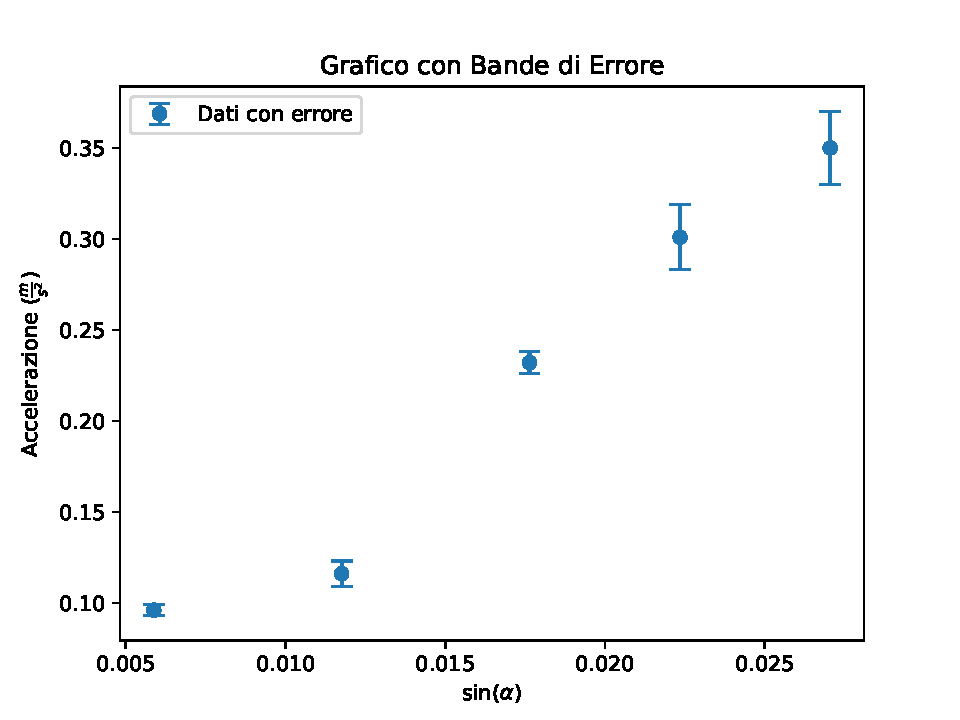
\includegraphics[width=1\textwidth]{grafico1p2.pdf}
  \caption{Grafico dei valori riportati in Tabella (9)}
\end{figure}

\section{Conclusione}
In conclusione notiamo che l'accelerazione in funzione del seno dell'inclinazione del piano segue un andamento fortemente non lineare. A causa dei pochi campioni analizzati non è possibile stimare una legge che leghi queste due variabili. Infatti, analizzando il grafico in Figura (8), possiamo notare che a causa dell'incertezza l'andamento può essere approssimato come una funzione esponenziale o come una radice. Dagli esperimenti e dalle varie misurazioni è stata verificata la validità della Legge (3).

\end{document}